\section{Evaluation}\label{sec:results}

%In this section, we will present our evaluation results of the \systemname. 
We evaluated \systemname~with comprehensive laboratory studies.
We collected from volunteer participants accelerometer sensor readings with Google Glass.
We analyzed these traces offline on a PC.
Our evaluations are primarily aimed at determining the accuracy of detecting 
and differentiating users based on their head-movements, and understand 
the effect of design parameters such as length of the music cue and training 
data-set size, on accuracy. We also report the response time of our Google 
Glass implementation of \systemname.
Our studies were approved by the Institutional Review Board (IRB) of our 
institution.
%based on profiling the execution time of each key 
%functions associated with \systemname, on the Google Glass device.

\iffalse
We conducted extensive evaluation of the Headbanger system. In particular, our 
evaluation focused on showing that a user's body movement pattern can be used 
to establish the user's identify. We first show that even a simple movement 
pattern is hard to imitate by others (i.e., being distinctive), and next show 
that people can easily repeat their own patterns (i.e., being repeatable). To 
conduct the evaluation, we prototyped the Headbanger system using the Google 
Glass, but our system can be easily implemented on other platforms.
\fi

%\begin{figure}[t]
%\centering
%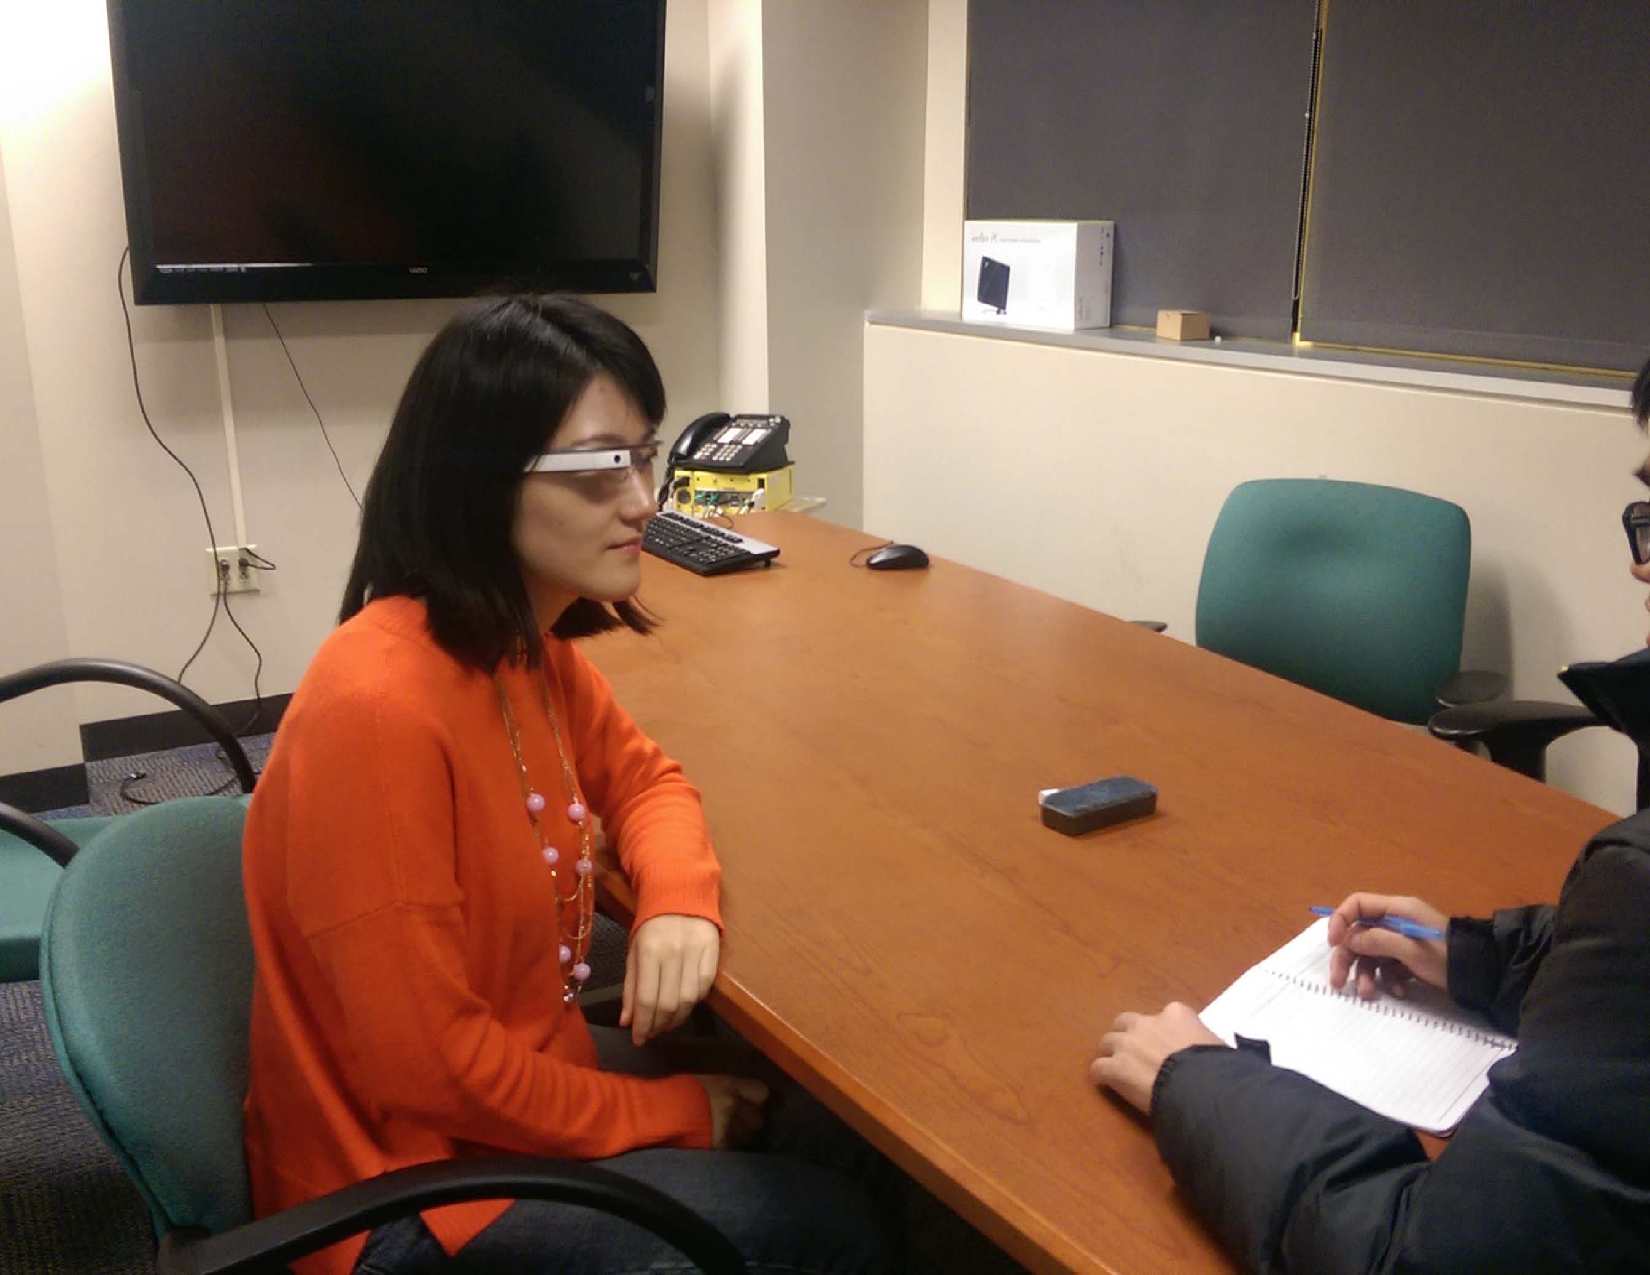
\includegraphics [width=.75\columnwidth]{../fig/exp.pdf}
%\caption{Our team member was collecting data with one of the participants. \label{fig:exp}}
%\end{figure}

\subsection{Method}
%\subsection{Dataset}



\paragraph{Participants}

We had total of 30 volunteer participants and did not include any of the 
authors. Table~\ref{tab:human-subjects-distrib} shows the distribution of the 
age and gender of the participants. The experiments were conducted by one of 
the authors, who demoed the usage to the subjects and proctored the trails.

\begin{table}[h]
\begin{tabular}{lclcl}
\cline{1-5}
       & \multicolumn{2}{c}{Male}                          & \multicolumn{2}{c}{Female}                             \\ \hline\hline
Gender & \multicolumn{2}{c}{19}                            & \multicolumn{2}{c}{11}                                 \\ \hline
       & \multicolumn{1}{l}{Mean} & \multicolumn{1}{l}{Mimimum}                & \multicolumn{1}{l}{Maxinum} & \multicolumn{1}{l}{Std Dev}                  \\ \hline\hline
Age    & \multicolumn{1}{c}{29.7}                     & \multicolumn{1}{c}{23} & \multicolumn{1}{c}{54}                          & \multicolumn{1}{c}{9.81} \\ \hline
\end{tabular}
\label{tab:human-subjects-distrib}
\caption{Participants gender and age distribution.}
\end{table}

\paragraph{Procedure}
Our experiment setup aimed at emulating the typical usage scenario 
of the \systemname~for authentication, where a user conducts head-movements in 
response to a music cue played on the Google Glass device during the login 
attempt.
In our experiment, all participants were asked to wear a Google Glass 
device. The device ran our data-collection app that played a piece of music 
(music cue) for a specific duration, and recorded the accelerometer sensor 
readings. We considered three duration values in our experiment: 5sec, 
6sec and 10sec. As we will discuss further, the accuracy of the system can 
significantly improve with the duration of the music cue; longer the duration 
better is the accuracy. 
The sensor readings were recorded into a text file that was stored 
in the Glass's memory and later transported to a PC for offline processing
through a Python script. The experiment was conducted in an well-lit indoor 
academic laboratory environment. 
 
The participants were allowed to take a break or withdraw from the 
experimentation if they felt uncomfortable at any point; for example, feeling 
dizzy after head-movement for a period of time, not being able to see clearly 
if near-sighted, etcetera. The conductor also allowed the user to take a break 
of about one minute after each experiment trial.
Each trial lasted for the duration of the music cue played on the Glass, and 
we conducted 40 trials for each of the 30 subjects. 
The experimentation was conducted over a duration of 60 days, where 20 
subjects conducted their trials in a single day over a period of two hours, 
while half of the trials of the rest 10 subjects were spread over 2 days.
The experiment yielded three sets of data traces that each correspond to 
the three music cue durations we selected. 
We will now discuss our evaluation results in detail.

\begin{figure}[t]
\centering
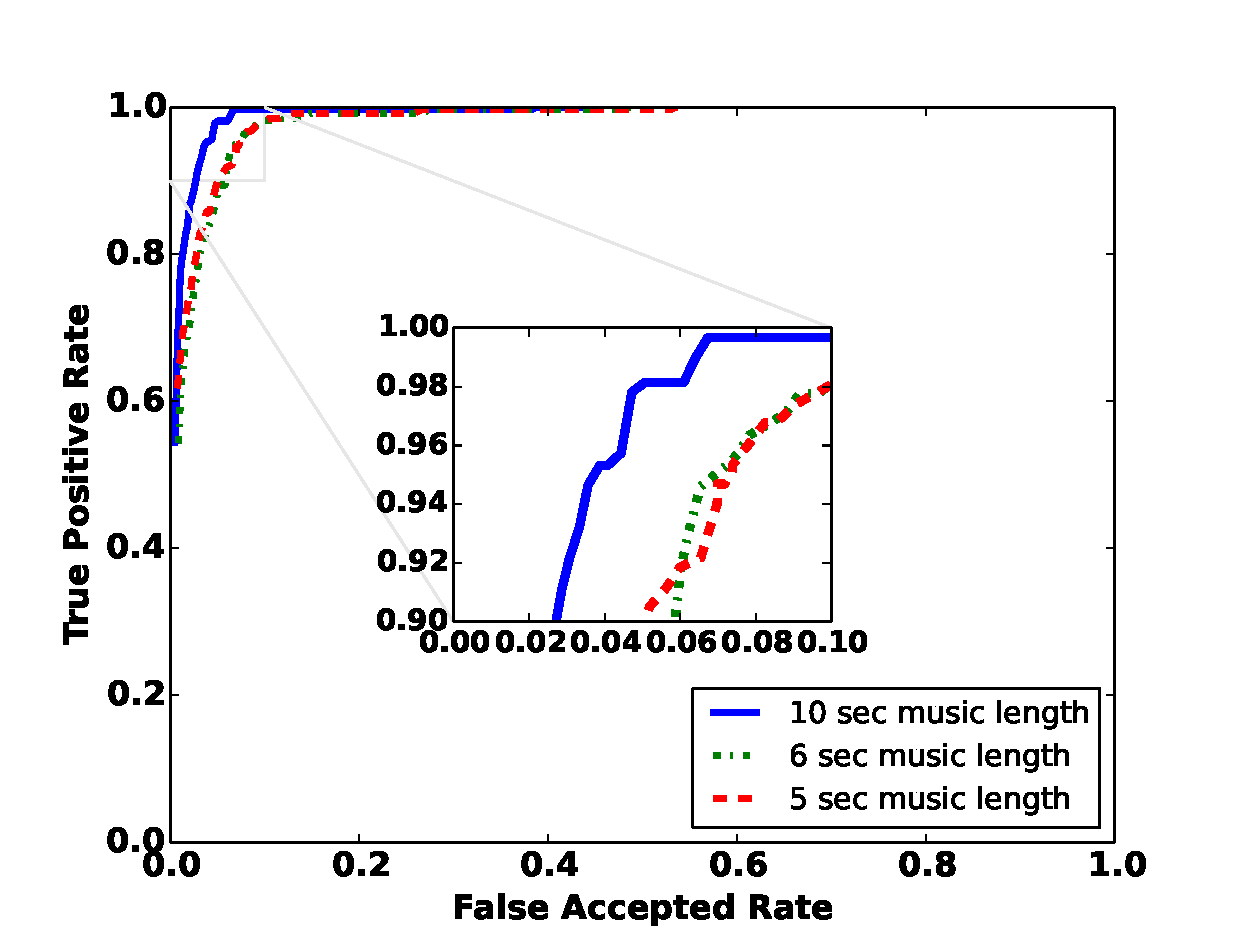
\includegraphics [width=.85\linewidth]{figure/top1_roc.eps}
\caption{Evaluation of music length impact on the accuracy in Top-1 scheme: the same music cue is trimmed into 10 sec, 6 sec, and 5 sec.}
\label{fig:roc-top1}
\end{figure}

\begin{figure}[t]
\centering
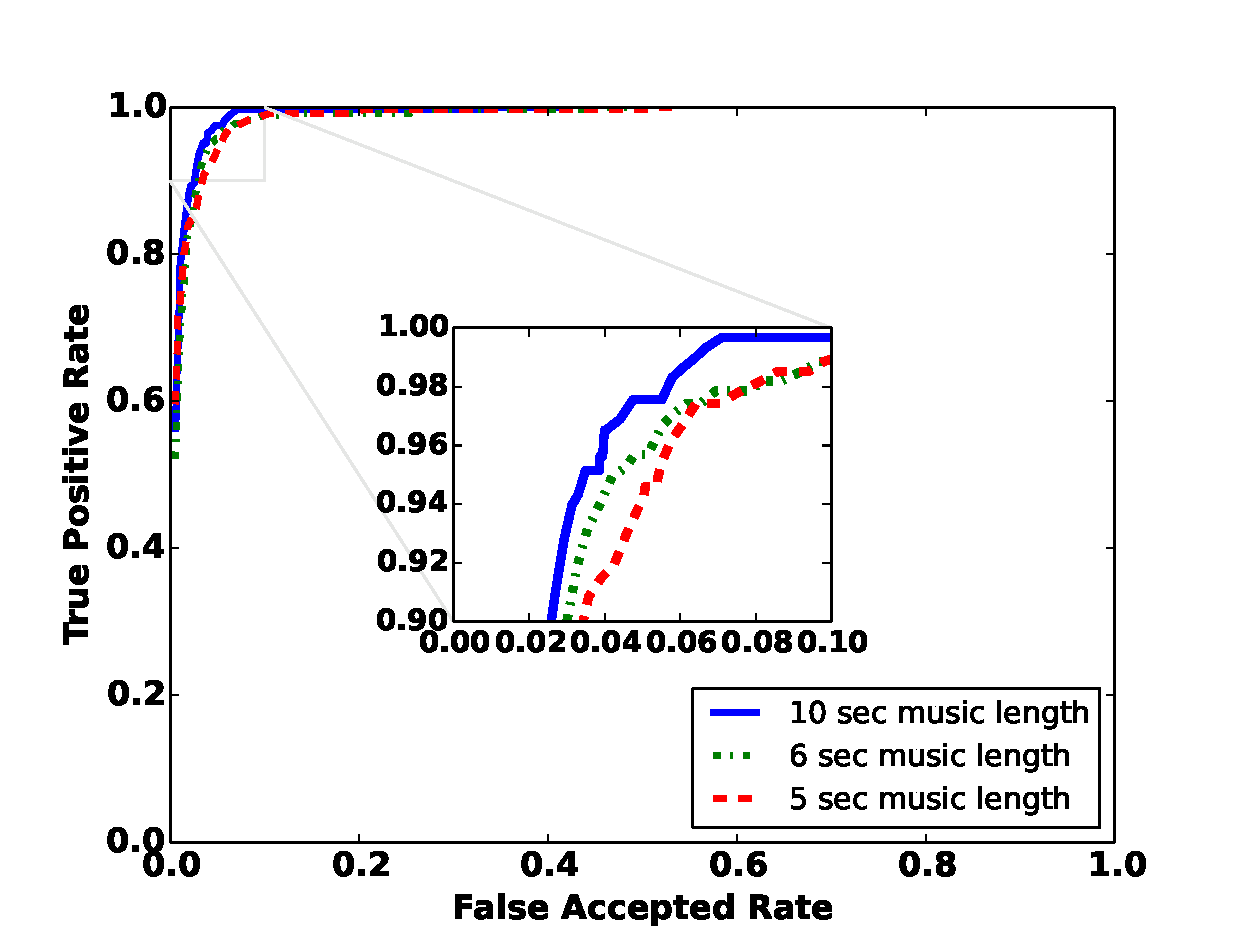
\includegraphics [width=.85\linewidth]{figure/top3_roc.eps}
\caption{Evaluation of music length impact on the accuracy in Top-3 Voting scheme: the same music cue is trimmed into 10 sec, 6 sec, and 5 sec.}
\label{fig:roc-top3}
\end{figure}

\begin{figure}[t]
\centering
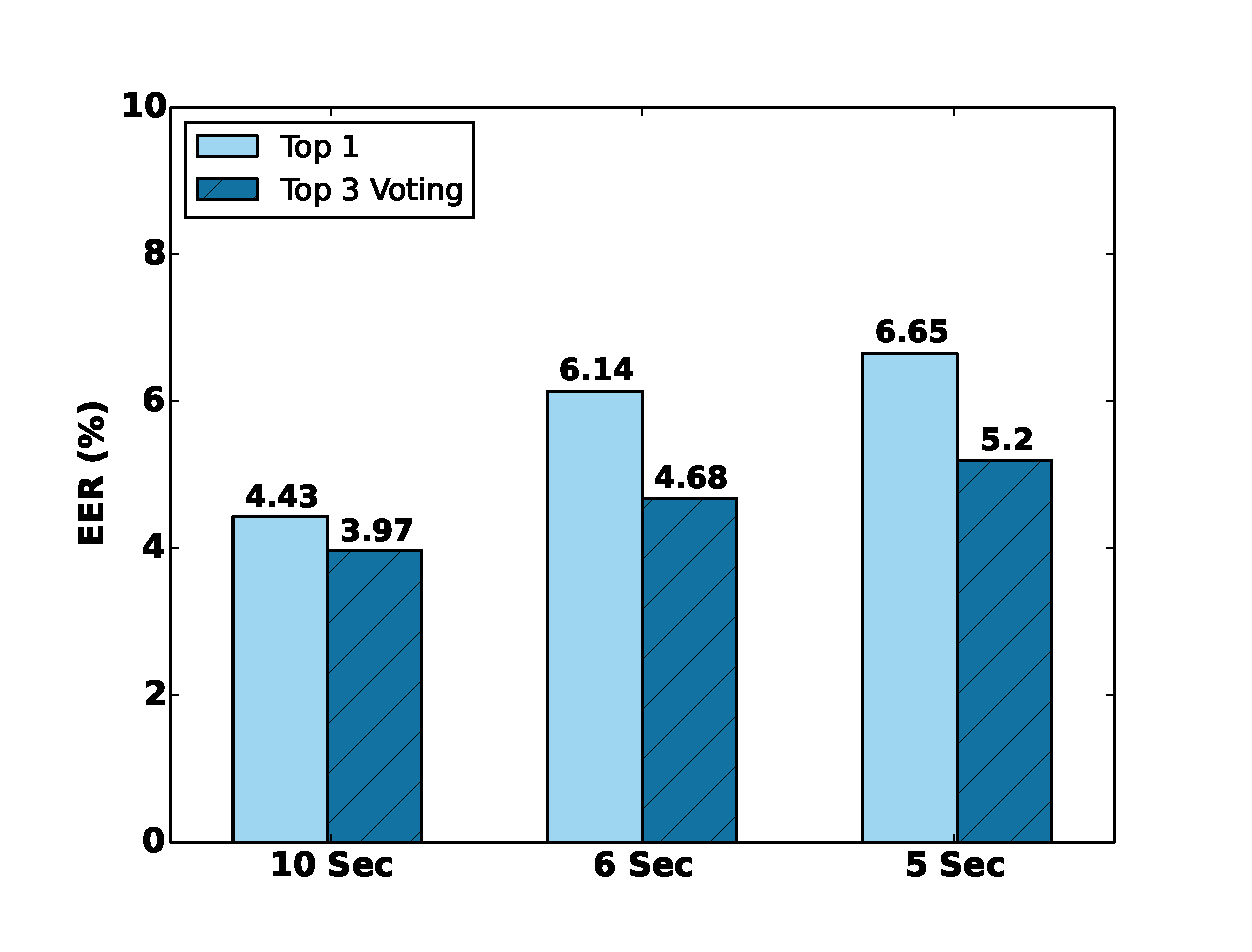
\includegraphics [width=.85\linewidth]{figure/exp2_vary_length.eps}
\caption{Comparison of EER for different music lengths (10 sec, 6 sec and 5 sec) with corresponded fixed n value}
\label{fig:eer-length}
\end{figure}

\begin{figure}[t]
\centering
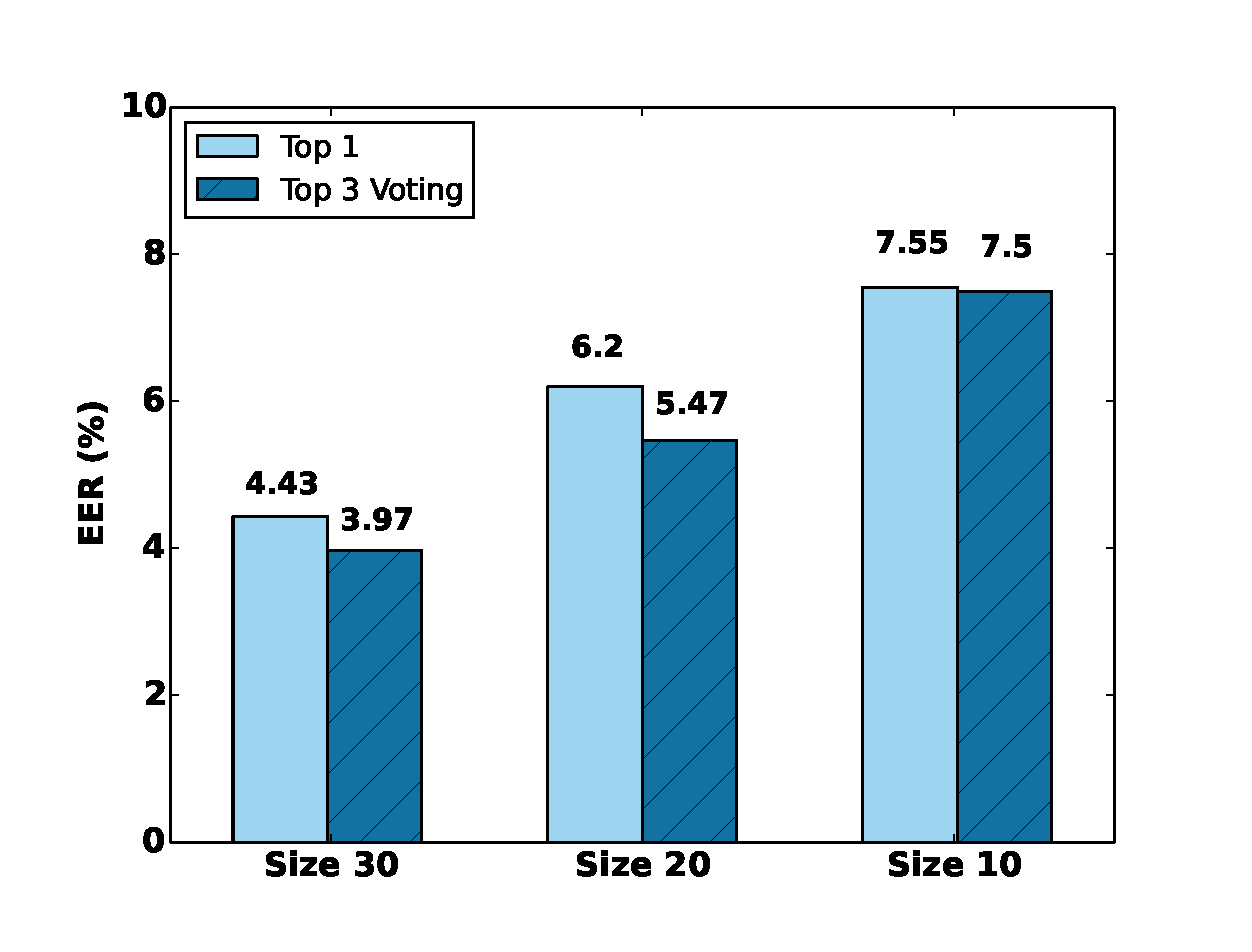
\includegraphics [width=.85\linewidth]{figure/exp2_vary_size.eps}
\caption{Comparison of EER for different training sample sizes (30, 20 and 10) with corresponded fixed n value}
\label{fig:eer-size}
\end{figure}

\subsection{Accuracy}
We evaluate the accuracy of \systemname~using metrics that are commonly used 
in evaluating authentication systems, namely,
the false acceptance rate FAR (percentage of false test samples that are 
mistakenly accepted), false rejection rate FRR (percentage of true test 
samples that are mistakenly rejected), and true positive rate 
TPR (percentage of true test samples that are correctly accepted). 
A strict threshold in the classifier can lead to high FRR, while 
overly relaxing the same can lead to a high FAR. Hence, we also consider 
metrics that combine both, particularly the equal error rate EER (percentage 
of errors when $FAR = FRR$).
%and balanced accuracy BAC, where BAC = 1 - (FAR+FRR)/2.
%We present the accuracy results through the receiver operating 
%characteristics (ROC) curves, TPR versus FAR, as shown in Figures~\ref{} 
%and~\ref{}. 
Figures~\ref{} report the accuracy of \systemname~through the metrics stated 
here. In general, our evaluation of the 30 subject data-set indicates that a 
TPR of 95$\%$ at FAR of 3$\%$, and EER = 3.97$\%$ can be achieved in 
\systemname with the following parameter choices:
10 sec music duration, $K = 3$, and 30 (out of 40) trials from each user being 
used for training with a $n=2.7$ (refer to section~\ref{}). 
We will now discuss the results and the impact of such parameter choices 
on accuracy in more detail.

\paragraph{Impact of $K$ value and music cue duration}
As discussed in section~\ref{sec:systemdesign}, our matching algorithm 
selects the match that has the minimum DTW distance from the top K 
features in the training set. We can observe from the ROC 
(receiver operating characteristic) curves in Figure~\ref{fig:roc-top1} and \ref{fig:roc-top3} that 
for both, $K=1$ and $K=3$, the TPR is close to 95$\%$ when the FAR is close to 
3$\$$ for the 10 sec music duration. For $K=1$ the FAR increases to 
about 7$\%$ for the 5 sec and 6 sec cases, however, by choosing $K=3$ the FAR 
decreases to about 3$\%$ and 4$\%$, respectively. 
We observe a similar trend with the EER as shown in Figure\ref{}; about 
0.5-1$\%$ improvements with $K=3$ compared to $K=1$.
This indicates that the accuracy in \systemname~improves with a larger value 
of $K$. However, the improvement in accuracy through redundancy in the 
training set trades off with the increased execution time as the 
matching now requires at least $K$ DTW computations. 
%We measure the DTW computation on Google Glass to be the most 
%computationally expensive operation of all the software modules in 
%\systemname.
%\paragraph{Impact of music cue duration}

In general, we observe from our results that the FAR can 
be decreased by increasing the music cue duration. 
We can observe that the improvements is less significant when the music cue
duration is increased from 5 sec to 6 sec, however the improvement is more 
significant when increased to 10 sec. 
In \systemname~the data input for the authentication system (the accelerometer 
sensor readings) is executed in parallel with the music cue.
We note that data input duration of 5-10 sec for authentication 
is on par with those of password based systems~\cite{}.
We also note that, since the authentication process is initiated only at the 
end of the music cue, execution time of the app will be independent
of this duration.

\paragraph{Impact of Training set size}
%The accuracy of detecting and matching the head-movements to the user depend 
%upon the music cue duration, value of $K$, and number of samples used for 
%training.
Recalling from section~\ref{sec:systemdesign}, the input to the training phase
is a set of temporal signals or samples (duration equal to the music cue 
duration), each corresponding to one trial of the head-movements from the 
user. Our evaluations so far considered a training set size of 30 samples. 
In Figure~\ref{}, we report the EER in \systemname~for three different 
training sizes; 10,20 and 30.
We can observe from Figure~\ref{} that the EER holds an inverse relationship 
with the training set size. A larger training set implies more confident mean 
and standard deviation values, as the errors in since the inconsistency in 
these values are reduced by averaging over a larger set of data.
A larger training set also implies a longer execution time of the training 
phase. We posit that the training phase can be conducted offline on a more
compute efficient device (smartphone, PC or server) and that the wearable
device can pre-fetch the trained data (for example, an XML file) prior to or 
during app execution through a wireless link.

%\paragraph{Effect of Imitation}

\subsection{Headbanger Google Glass App Implementation}

\begin{table}
\small\centering
\begin{tabular}{|l|l|}\hline
Music sample duration (s) & processing latency (s) \\\hline
5 & 2.44\\\hline
6 & 2.73 \\\hline
10 & 4.47 \\\hline
\end{tabular}
\caption{Measured processing latencies on Google Glass with different sample 
durations. We generated the results using Top 1 testing for thresholding based 
classification.
\label{tab:glass}}
\end{table}

We implemented the \systemname~authentication app on Google glass. 
Figure~\ref{fig:software_arch} shows the software modules in the app.
Upon initiation by the user the app plays a music cue for a stipulated 
duration. The user conducts head-movements in synchrony with the music cue 
while the app records the accelerometer sensor in parallel. At the end of the 
music cue duration the app executes the authentication process where the 
sensor readings are input to the \systemname~software modules. The 
\systemname~modules extract the head-movement features through the 
thresholding process discussed in section~\ref{sec:systemdesign}, and compare 
with the feature templates generated from the training phase. The app responds 
with a YES or NO textual output on the Google Glass screen, depending on the 
match.
In our current implementation, we conduct the training phase offline, prior to 
live-testing of the app, generate the features and save them into the server. 
We pre-fetch the training data-set from the server when the app is fired, so 
that the training set is readily available during the authentication process, 
thus decreasing the processing latency.
%Among all the software modules, the ``training set construction model'' is 
%the most computing-intensive, and as a result, we executed the model on the 
%bluetooth-paired smartphone. The rest of the modules are implemented and 
%executed on the glass. 
%In our on-glass app, the classification module runs the 
%thresholding-based classification. 
Table~\ref{tab:glass} shows the measured 
response-time (time between music cue completion to YES/NO response on the 
screen) of the \systemname Google Glass app. 
Our measurements indicate that the response times are in the order few seconds 
in our current implementation. Based on profiling the execution time of each 
module we also observed that (as shown in Table~\ref{tab:glass}) the most 
compute intensive task is the DTW computation. In our current implementation 
we used a faster version of the DTW algorithm called Fast DTW~\cite{}**SUGANG, 
and 
we hope that the execution time can be reduced further through optimizations 
in the algorithm. However, we feel that a response time of 1-4sec for a local 
authentication solution in Google Glass is comparable to that of the solutions 
and implementations so far~\cite{}**SUGANG.



\iffalse
\subsection{Controlled Experiments: Can You Repeat Your Body Movement?}\label{sec:experiment1}
We first investigate the consistency of the movement performed by each subject. Physical biometric such as fingerprint and iris, which are permanent characteristics that remains regardless environment, emotion, and time. However, behavioral biometric is combined with human controllable movement
\fi

